%!TEX root = ../PTC-LibUG.tex

\chapter{Linking Magnets Together and Moving Them as a Group}
\label{cha:girders}

\fxnote{Review underscore (\_\,) characters in index entries.}
\fxnote{Review percent (\%\,) characters in index entries.}
\fxnote{Review line numbers.}
\fxnote{Say something re misalign v. translate or move. (Or do this in \Cref{geometry}.)}

\index{magnets!linking together}
\index{magnets!moving as group}
\index{Large Hadron Collider!bore magnets}
\index{LHC|see{Large Hadron Collider}}
%
In many accelerator designs, there are groups of elements that move
together as a unit. The Large Hadron Collider, for example, has
dual-bore magnets that carry the two counter-propagating beams through
the cryostats. A more common example is a group of elements assembled
onto a single substrate. When misalignments are applied to
such units, our accelerator modeling code should respect the internal
geometric constraints.

\PTC\ allows us to link elements together to model groups of elements
that move as units. In this chapter, we describe the two tools that
\PTC\ provides---called siamese and girders---and we illustrate their
use by applying them to the collider (layouts \ptc{Col1} and \ptc{Col2})
of the previous chapter.


\section{Siamese and Girders}
\label{sec:siamese.girders}

\index{siamese!defined}
\index{magnet!siamese}
\index{linked list!circular}
\index{siamese!misaligning}
\index{misalignment!siamese}
\index{siamese!frame of reference}
%
A \emph{siamese} consists of elements that are linked together so
that one can move them as a group. Those elements may be in the
same or different layouts. The elements in a siamese are often
parallel, as in a collider; but they may be in different arcs of
a recirculator---arcs, for example, that share common cryogenics.

\begin{marginfigure}[3\baselineskip]\forcerectofloat
  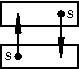
\includegraphics{SiameseGirders/siamgird-01}
  \caption{A pair of elements linked together as a siamese.}
  \label{fig:ll.siamese}
\end{marginfigure}

\begin{marginfigure}
  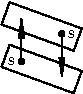
\includegraphics{SiameseGirders/siamgird-02}\quad
  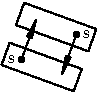
\includegraphics{SiameseGirders/siamgird-03}
  \caption{Incorrect and correct rotations of a siamese.}
  \label{fig:siamese.rot}
\end{marginfigure}

To create a siamese, we build a circular linked list containing
the several elements we wish to tie together. See \fref{ll.siamese}.
When moving a siamese, \PTC\ traverses the linked list, moving
all the siamese elements in concert. Note that doing this
properly---\ie\ preserving the geometric relations between the
siamese elements---requires the use of a common reference frame.
\fref[c]{siamese.rot}, for example, illustrates incorrect and correct rotations of a pair of elements linked together as a siamese.
In the left-hand graphic of that figure, the same rotation applied
to the \emph{separate} elements breaks the geometry of the siamese.
In the right-hand graphic, the use of a common reference frame when
rotating the elements preserves the geometry. When we link the
elements together as a siamese and then ask \PTC\ to rotate the
siamese---as opposed to the individual elements---\PTC\ takes care
of the details and preserves the internal geometric constraints.
We discuss geometric operations applied to siamese later in this
chapter. See also \TPref*{sec:ops.siamese}.

A siamese does not have an independent reference frame; instead, a
siamese frame is defined in terms of translations and rotations with
respect to the frame of one of its constituent elements. Misalignments
of a siamese are then specified in a similar way with respect to the
siamese frame. If we zero the misalignments, the siamese returns to
its original location.

\index{girder!defined}
\index{magnet!in girder}
\index{girder!misaligning}
\index{misalignment!girder}
\index{girder!frame of reference}
\index{affine\_frame@\ptc{affine\_frame}}
%
A \emph{girder} is a collection of siamese and regular elements
tied to a substrate so that one can move them as a unit. Like a
siamese, we construct a girder as a circular linked list containing
the elements belonging to the common substrate. See \fref{ll.girder}.
Unlike a siamese, a girder typically has its own reference frame,
independent of any element on the girder. This is actually a
\emph{pair} of reference frames---stored in the \PTC\ data type
\ptctyp{affine_frame}. The two frames specify location and
orientation for the original and misaligned girder. This structure
simplifies the process of misaligning a girder: If applying a
\emph{different} misalignment to the girder, \PTC\ starts with
the original frame. If \emph{adding} to an existing misalignment,
\PTC\ uses the misaligned frame as its starting point. If we remove
the misalignment, \PTC\ easily returns the girder to its original
position in the lattice. We discuss geometric operations applied
to girders later in this chapter. See also \TPref*{sec:ops.girders}.

\begin{marginfigure}[-21\baselineskip]\forceversofloat
  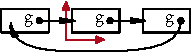
\includegraphics{SiameseGirders/siamgird-04}
  \caption{A trio of elements linked together as a girder that
           has its own reference frame.}
  \label{fig:ll.girder}
\end{marginfigure}

Do note that linking together a group of elements on a girder does not mean those elements may no longer move with respect to one another. It is only the geometric operations that apply specifically to girders that will preserve the geometric relations between the girder elements. A similar comment applies for the siamese.

\index{PTC!source file}
\index{source file!geometry tutorial}
\index{geometry!tutorial source file}
\index{z\_ptc\_geometry.f90@\ptc{z\_ptc\_geometry.f90}!geometry tutorial source file}
\index{siamese!creating}
\index{girder!creating}
\index{siamese!misaligning}
\index{misalignment!siamese}
\index{girder!misaligning}
\index{misalignment!girder}
%
In this chapter we show how to create a pair of siamese and a girder
in the collider---trackable layouts \ptc{Col1} and \ptc{Col2} from
\Cref{model.accel}---as well as how to misalign them. The code in
this chapter is from the \PTC\ geometry tutorial source file,
\ptc{ptc_geometry.f90}, which is given in \Aref{geom.tutorial}.
The line numbers of the code shown here refer to the line numbers
of the code in that appendix.


\section{Building Siamese, Girders, and their Reference Frames}

\begin{marginfigure}[2\baselineskip]\forceversofloat
  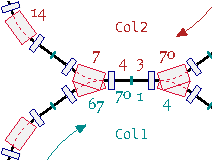
\includegraphics[]{Layouts/models-08}
  \caption{Collider interaction region. The numbers show the indices
           of a few of the fibres within the corresponding layout.}
  \label{fig:col.intxn}
\end{marginfigure}

\index{move\_to@\ptc{move\_to}!routine}
\index{routine!\ptc{move\_to}}
%
At each end of the straight section shared by layouts \ptc{Col1}
and \ptc{Col2}, see \fref{col.intxn}, is a pair of overlapping bend
magnets. In the first block of code below, we group each pair of bends
as a siamese. For the pair at the left-hand end of the straight,
we set, in the first two lines, pointers \ptc{p1} and \ptc{p2}
respectively to the 67$^\text{th}$ and 7$^\text{th}$ fibres of
layouts \ptc{Col1} and \ptc{Col2}. Those two fibres contain the
pair of elements we wish to group together as a siamese. Each of
those elements---\ptc{p1\%mag} and \ptc{p2\%mag}---contains an
element pointer called \ptc{siamese}. In \lref[s]{siam1.p2} and
\lref*{siam2.p1} we now set each element's \ptc{siamese} pointing
to the other element, thus creating a circular linked list that
ties these two elements together.

In a similar fashion, the next four lines link together as a
siamese the two bends at the right-hand end of the common straight.
Those elements belong to the 4$^\text{th}$ and 70$^\text{th}$
fibres respectively of layouts \ptc{Col1} and \ptc{Col2}.
%
\setptclinenums{386}{5}
\begin{ptccode}
call move_to(Col1, p1, 67)
call move_to(Col2, p2, 7)
p1%mag%siamese => p2%mag    \label{lin:siam1.p2}
p2%mag%siamese => p1%mag    \label{lin:siam2.p1}
call move_to(Col1, p1, 4)
call move_to(Col2, p2, 70)
p1%mag%siamese => p2%mag
p2%mag%siamese => p1%mag
\end{ptccode}

\enlargethispage{\baselineskip}
Our next goal is to group together onto a girder the above two
siamese and all the intervening elements shared by layouts
\ptc{Col1} and \ptc{Col2}. In addition, we will add one more
element to our girder: the bend in the 14$^\text{th}$ fibre of
layout \ptc{Col2} (see upper left of \fref{col.intxn}). We do
this not because this example seems likely from an engineer's
perspective, but because we want to illustrate the flexibility
of \PTC's approach. In particular, we wish to emphasize the
fact that elements tied to a common girder need not be adjacent.
Nevertheless, tied to a common substrate, they will move as a unit.

The next block of code links together the elements we want on our girder. As for the case of siamese, every \PTC\ \ptctyp{element} contains an element pointer called \ptc{girders}, and we use this to construct the linked list that ties our girder elements together. Pointing \ptc{p1} to the short drift at the left-hand end of the common straight section (in fibre~68 of layout \ptc{Col1}), we deal first with the girder elements common to layouts \ptc{Col1} and \ptc{Col2}. In \lref[s]{blp.grdr}--\lref*{elp.grdr}, we march along the straight section, pointing \ptc{p2} to the next fibre, linking the elements in \ptc{p1} and \ptc{p2} (\lref{link.lp}), and then advancing \ptc{p1}. After that loop terminates, both \ptc{p1} and \ptc{p2} point to fibre~4 in layout \ptc{Col1}, and we have linked together the elements of the common straight section plus that last bend.
%
\begin{ptccode}
call move_to(Col1, p1, 68)
pf => p1  ! remember start of girder linked-list
do i = 2, 7                 \label{lin:blp.grdr}
  p2 => p1%next
  p1%mag%girders => p2%mag  \label{lin:link.lp}
  p1 => p1%next
end do                      \label{lin:elp.grdr}
call move_to(Col2, p2,  7)
p1%mag%girders => p1%mag%siamese  \label{lin:grdr.4.70}
p1%mag%siamese%girders => p2%mag  \label{lin:grdr.70.7}
p2%mag%girders => p2%mag%siamese  \label{lin:grdr.7.67}
call move_to(Col1, p1, 67)
call move_to(Col2, p2, 14)
p1%mag%girders => p2%mag          \label{lin:grdr.67.14}
p2%mag%girders => pf%mag           \label{lin:grdr.14.68}
\end{ptccode}
%
In the rest of this block of code, we link in the remaining four
bends we want on our girder: the ones labeled 7, 14, and 70 from
\ptc{Col2}, and 67 from \ptc{Col1}. (Because these four labels are
distinct, we
simplify the following description: instead of saying, for example,
``the bend in fibre~4 of \ptc{Col1}'', we shall say simply ``bend~4''.)
First, we move \ptc{p2} to bend~7. \lref[c]{grdr.4.70} then links
bend~4 to bend~70, because \ptc{p1\%mag\%siamese} already points to
the latter. \lref[c]{grdr.70.7} links bend~70 to bend~7; and
\lref{grdr.7.67} links bend~7 to bend~67, because \ptc{p2\%mag\%siamese}
already points to the latter. It now remains for us to link in
bend~14 and then close our linked list of girder elements. To do
this, we first point \ptc{p1} to bend~67 and \ptc{p2} to bend~14.
Then \lref{grdr.67.14} adds the girder link from one to the other
of those two elements. Finally, \lref{grdr.14.68} closes the linked
list.

We now have a pair of siamese and a girder defined in our collider.
Our next task is to define appropriate siamese and girder frames.
Though we may locate those frames wherever we wish, a sensible choice
for the girder might be to make it coincide with the entrance frame
of the first fibre in layout \ptc{Col1}, at the center of our collider's
common straight section. We accomplish this in the next block of
code.

\index{allocate\_af@\ptc{allocate\_af}!routine}
\index{routine!\ptc{allocate\_af}}
\index{girder\_frame@\ptc{girder\_frame}}
%
\enlargethispage{\baselineskip}
After moving \ptc{p1} to the first fibre in layout \ptc{Col1}, we
then, in \lref{alloc.gf}, allocate memory for the special dual
reference frame needed by our girder, \ptc{p1\%mag\%girder_frame}.%
\sidenote[][-7.5\baselineskip]{Read \ptc{alloc\_af} as ``allocate affine frame''.}
This has four pieces we need to define: \ptc{a} and \ptc{b} for
the origins of the original and current (or misaligned) frames,
and \ptc{ent} and \ptc{exi} for the bases of those two frames.%
\sidenote[][-7.5\baselineskip]{Here the \emph{origin} of a reference
frame refers to a three-dimensional vector that stores the
co\"ordinates of the local frame's origin with respect to the
global frame. The \emph{basis} refers to a $3\times3$ matrix whose
rows contain the orthogonal unit vectors of the local frame, written
with respect to the global frame. See \Cref{geometry} for more details.}
In the remaining four lines of this block of code, we set these
components equal to the corresponding parts (origin or basis) of
the entrance reference frame of the element in fibre \ptc{p1}.
This information is held in \ptc{p1\%mag\%parent_fibre\%chart\%f},
which you might read as ``the magnet frame attached to the chart
associated with this element's parent fibre''.
%
\begin{ptccode}
call move_to(Col1, p1, 1)
call alloc_af(p1%mag%girder_frame, girder = .true.)  \label{lin:alloc.gf}
p1%mag%girder_frame%a   = p1%mag%parent_fibre%chart%f%a
p1%mag%girder_frame%ent = p1%mag%parent_fibre%chart%f%ent
p1%mag%girder_frame%b   = p1%mag%parent_fibre%chart%f%a
p1%mag%girder_frame%exi = p1%mag%parent_fibre%chart%f%ent
\end{ptccode}
%
As set here, the original and current frames are identical,
so this girder is in its design location. Later, if we ask
\PTC\ to misalign this girder, it will modify \ptc{girder_frame\%b}
and \ptc{girder_frame\%exi}, leaving \ptc{girder_frame\%a} and
\ptc{girder_frame\%ent} to record the design location and
orientation of our girder.

\begin{marginfigure}[2\baselineskip]
  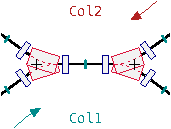
\includegraphics{Layouts/models-09}
  \caption{Collider interaction region. The small cross-hairs
           indicate the frame location for each siamese.}
  \label{fig:col.siamfr}
\end{marginfigure}

\index{siamese\_frame@\ptc{siamese\_frame}}
%
In the following block of code, we also define reference frames for
the two siamese. In this case, we choose to locate the siamese frames
along the axis of the common straight section, five meters from the
center of that straight, and oriented parallel to the girder's frame of
reference. (See the cross-hairs in \fref{col.siamfr}.) Consider first
the left-hand siamese: We compute, in \lref[s]{sf.borg}--\lref*{sf.eorg},
the desired origin of our siamese frame. Then, in the following two
lines, we move fibre pointer \ptc{p3} to bend~67 and allocate the
necessary memory.%
\sidenote{This means the siamese frame will be attached to bend~67,
but one could equally well attach it to bend~7, the other magnet in
this siamese.}
Here is where a siamese and girder differ. When \PTC\ allocates a
\emph{girder} frame (by setting \ptc{girder = .true.}, as in
\lref{alloc.gf} above), it allocates memory for the data \ptc{a},
\ptc{ent}, \ptc{b}, and \ptc{exi}. For the siamese frame (the default, as in
\lref{alloc.sf} below,  is \ptc{girder = .false.}) \PTC\ allocates
memory for the data \ptc{d} and \ptc{angle}, which specify not the
frame itself, but rather how to get there (translation and angle)
from the entrance frame of the local element. Our next step is
therefore to compute \ptc{d} and \ptc{angle}. This we do in
\lref{sf.patch} with a call to \ptc{find\_patch}. The first two
arguments are respectively the origin and basis of bend~67's entrance
frame. The second two arguments are the desired origin (\ptc{a}) and
basis (same as for the girder). And the last two arguments are
the computed translation and angle, which we store in our siamese
frame: \ptc{p3\%mag\%siamese_frame\%d} and
\ptc{p3\%mag\%siamese_frame\%angle}.

In a similar fashion, the remaining lines in this block of code
define the reference frame for the other siamese.
%
\begin{ptccode}
a = p1%mag%girder_frame%a                         \label{lin:sf.borg}
a(3) = a(3) - 5.d0                                \label{lin:sf.eorg}
call move_to(Col1, p3, 67)
call alloc_af(p3%mag%siamese_frame)               \label{lin:alloc.sf}
call find_patch(p3%mag%p%f%a, p3%mag%p%f%ent, &   \label{lin:sf.patch}
                a, p1%mag%girder_frame%ent, &
                p3%mag%siamese_frame%d, p3%mag%siamese_frame%angle)
a = p1%mag%girder_frame%a
a(3) = a(3) + 5.d0
call move_to(Col1, p3, 4)
call alloc_af(p3%mag%siamese_frame)
call find_patch(p3%mag%p%f%a, p3%mag%p%f%ent, &
                a, p1%mag%girder_frame%ent, &
                p3%mag%siamese_frame%d, p3%mag%siamese_frame%angle)
\end{ptccode}


\section{Examples of Misalignments}
\label{sec:xmpl.misalign}

The remaining blocks of code in this chapter show some examples of
misalignment operations on the girder and siamese---with variations
in their order and options. In the margin are corresponding figures
that illustrate the effect of the different misalignments. (For
comparison, \fref{col.nomis} shows the same portion of the collider
with no misalignments.) To make the effects clear, we have made very
exaggerated ``misalignments'':
$\SI{\piunit/8}{\radian} = \ang{22.5}$ for rotations, and \SI{2}{m}
for displacements.

The various misalignments are specified by the six-component vector
\ptc{mis}: the first three components describe translation, while
the last three describe rotation in \PTC\ order. This code is
probably only somewhat self-explanatory. Nevertheless, we present
it here for you to look at and mull over, with only a little in the
way of comments. A detailed explanation is given in \CTref*{geometry}.

\begin{marginfigure}[5\baselineskip]\forcerectofloat
  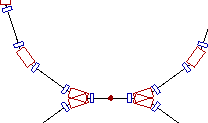
\includegraphics{SiameseGirders/siamgird-mma-0}
  \caption{No misalignment.}
  \label{fig:col.nomis}
\end{marginfigure}

Concerning \lref{moveto.b7}, note that bend~7 (\ie\ the bend contained
in fibre~7 of layout \ptc{Col2}) is present in both the girder and the
left-hand siamese, which are the parts we misalign in the examples
given here. That bend is not \emph{directly} associated with either
the girder frame or the siamese frame. But it is \emph{in}directly
associated: via the linked lists that define the girder and the
siamese, \PTC\ can always find the appropriate girder or siamese frame.
%
\index{misalign\_siamese@\ptc{misalign\_siamese}!routine}
\index{routine!\ptc{misalign\_siamese}}
\index{misalign\_girder@\ptc{misalign\_girder}!routine}
\index{routine!\ptc{misalign\_girder}}
%
\begin{ptccode}
write(6,*) "Example # (from the manual) 1--11 ?"
read(5,*) example
call move_to(Col2, p2, 7) \label{lin:moveto.b7}
if(example == 1) then            \textcolor{DarkRed}{\textsl{! Example 1}}
  mis = 0.d0
  mis(5) = pi / 8.d0
  call misalign_girder(p2, mis)
elseif(example == 2) then        \textcolor{DarkRed}{\textsl{! Example 2}}
  mis = 0.d0
  mis(1) = 2.0d0
  call misalign_girder(p2, mis)
elseif(example == 3) then        \textcolor{DarkRed}{\textsl{! Example 3}}
  mis = 0.d0
  mis(5) = pi / 8.d0
  call misalign_girder(p2, mis)
  mis = 0.d0
  mis(1) = 2.d0
  call misalign_girder(p2, mis, add = .false.)
elseif(example == 4) then        \textcolor{DarkRed}{\textsl{! Example 4}}
  mis = 0.d0
  mis(5) = pi / 8.d0
  call misalign_girder(p2, mis)
  mis = 0.d0
  mis(1) = 2.d0
  call misalign_girder(p2, mis, add = .true.)
elseif(example == 5) then        \textcolor{DarkRed}{\textsl{! Example 5}}
  mis = 0.d0
  mis(1) = 2.d0
  mis(5) = pi / 8.d0
  call misalign_girder(p2, mis)
\end{ptccode}

\begin{marginfigure}[-13.1cm]\forcerectofloat
  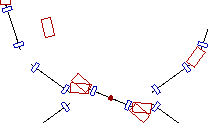
\includegraphics{SiameseGirders/siamgird-mma-1}%
  \makebox[0pt]{\textcolor{DarkRed}{1}}\\[14pt]\noindent
  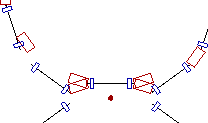
\includegraphics{SiameseGirders/siamgird-mma-2}%
  \makebox[0pt]{\textcolor{DarkRed}{2}}\\[14pt] \noindent
  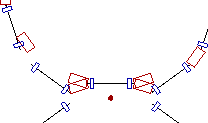
\includegraphics{SiameseGirders/siamgird-mma-3}%
  \makebox[0pt]{\textcolor{DarkRed}{3}}\\[14pt] \noindent
  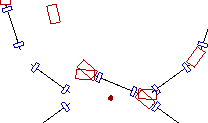
\includegraphics{SiameseGirders/siamgird-mma-4}%
  \makebox[0pt]{\textcolor{DarkRed}{4}}\\[14pt] \noindent
  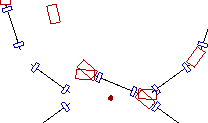
\includegraphics{SiameseGirders/siamgird-mma-5}%
  \makebox[0pt]{\textcolor{DarkRed}{5}}
  \caption{Examples 1 (top) through 5 (bottom).}
\end{marginfigure}

The examples above all misalign only the girder. In the following examples, we apply a misalignment also to one of the siamese. Note that the difference between examples 7 and 8 is solely to the optional argument \ptc{add} in \lref[s]{mis.x7} and \lref*{mis.x8}.
%
\begin{ptccode}
elseif(example == 6) then        \textcolor{DarkRed}{\textsl{! Example 6}}
  mis = 0.d0
  mis(1) = 2.d0
  call misalign_siamese(p2, mis)
elseif(example == 7) then        \textcolor{DarkRed}{\textsl{! Example 7}}
  mis = 0.d0
  mis(1) = 2.d0
  call misalign_siamese(p2, mis)
  mis = 0.d0
  mis(1) = 2.d0
  mis(5) = pi / 8.d0
  call misalign_girder(p2, mis, add = .false.) \label{lin:mis.x7}
elseif(example == 8) then        \textcolor{DarkRed}{\textsl{! Example 8}}
  mis = 0.d0
  mis(1) = 2.d0
  call misalign_siamese(p2, mis)
  mis = 0.d0
  mis(1) = 2.d0
  mis(5) = pi / 8.d0
  call misalign_girder(p2, mis, add = .true.) \label{lin:mis.x8}
elseif(example == 9) then        \textcolor{DarkRed}{\textsl{! Example 9}}
  mis = 0.d0
  mis(1) = 2.d0
  mis(5) = pi / 8.d0
  call misalign_girder(p2, mis)
  mis = 0.d0
  mis(1) = 2.d0
  call misalign_siamese(p2, mis, add = .false.)
elseif(example == 10) then       \textcolor{DarkRed}{\textsl{! Example 10}}
  mis = 0.d0
  mis(1) = 2.d0
  mis(5) = pi / 8.d0
  call misalign_girder(p2, mis)
  mis = 0.d0
  mis(1) = 2.d0
  call misalign_siamese(p2, mis, add = .true.)
elseif(example == 11) then       \textcolor{DarkRed}{\textsl{! Example 11}}
  mis = 0.d0
  mis(1) = 2.d0
  mis(5) = pi / 8.d0
  call misalign_girder(p2, mis)
  mis = 0.d0
  mis(1) = 2.d0
  call misalign_siamese(p2, mis, add = .false., &
                        preserve_girder = .true.)
end if
\end{ptccode}

\begin{marginfigure}[-17.3cm]\forceversofloat
  \makebox[0pt][l]{\textcolor{DarkRed}{6}}%
  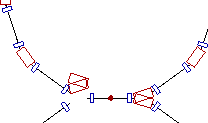
\includegraphics{SiameseGirders/siamgird-mma-6}\\[24pt]\noindent
  \makebox[0pt][l]{\textcolor{DarkRed}{7}}%
  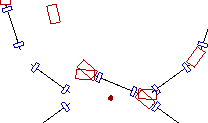
\includegraphics{SiameseGirders/siamgird-mma-7}\\[24pt]\noindent
  \makebox[0pt][l]{\textcolor{DarkRed}{8}}%
  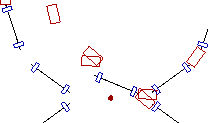
\includegraphics{SiameseGirders/siamgird-mma-8}\\[24pt]\noindent
  \makebox[0pt][l]{\textcolor{DarkRed}{9}}%
  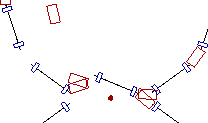
\includegraphics{SiameseGirders/siamgird-mma-9}\\[24pt]\noindent
  \makebox[0pt][l]{\textcolor{DarkRed}{10}}%
  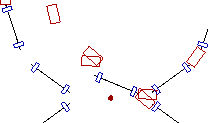
\includegraphics{SiameseGirders/siamgird-mma-10}\\[24pt]\noindent
  \makebox[0pt][l]{\textcolor{DarkRed}{11}}%
  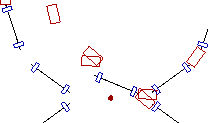
\includegraphics{SiameseGirders/siamgird-mma-11}
  \caption{Examples 6 (top) through 11 (bottom).}
\end{marginfigure}


\endinput
